\documentclass[aspectratio=169]{beamer}

%---------------------------
%       Beamer Cheat Sheet
%---------------------------
% https://www.cpt.univ-mrs.fr/~masson/latex/Beamer-appearance-cheat-sheet.pdf

%---------------------------
%       Set Theme and Colors
%---------------------------

\usetheme[width=.1\paperwidth]{Hannover}
% \setbeamertemplate{sidebar canvas right}[vertical shading][top=red,bottom=blue]

\definecolor{QESblue}{HTML}{8AD2ED}
\definecolor{QESdarkblue}{HTML}{187ca2}
\definecolor{QESlightblue}{HTML}{c4e8f6}

\setbeamercolor{sidebar}{bg=QESlightblue}
\setbeamercolor{titlelike}{fg=QESdarkblue}

\setbeamercolor{palette sidebar secondary}{fg=QESdarkblue}
\setbeamercolor{title in sidebar}{fg=QESdarkblue}
\setbeamercolor{author in sidebar}{fg=QESdarkblue}

\addtobeamertemplate{sidebar left}{}{\vfill \hspace{.006\paperwidth} 
\includegraphics[width=.08\paperwidth]{../../../logo.png} \vspace{.006\paperwidth} } 
% \addtobeamertemplate{sidebar left}{}{\vfill \hspace{.00001\paperwidth} 
\includegraphics[width=.093\paperwidth]{../../figures/qes-qr.png} \vspace{.003\paperwidth} } 

%---------------------------
%       No navigation symbols
%---------------------------
\setbeamertemplate{navigation symbols}{}

%---------------------------
%       Set Fonts
%---------------------------
\usepackage{helvet}
\renewcommand{\familydefault}{\sfdefault}
\usepackage{sansmathfonts}
\usepackage{upgreek}

\setbeamerfont{frametitle}{series=\bfseries, size=\Large}
\setbeamerfont{title in sidebar}{series=\bfseries, size=\small}
\setbeamertemplate{caption}{\it\raggedright\insertcaption\par}

%---------------------------
%       Math font packages
%---------------------------
\usepackage{dsfont, amsmath, amsthm, mathtools}
\usepackage{bbm, bm}
\usepackage[T1]{fontenc}
\usepackage[version=3]{mhchem}

%---------------------------
%       Figure packages
%---------------------------
\usepackage{graphicx}
\graphicspath{{../../figures}}

\usepackage{epstopdf}
\usepackage{color}

\setbeamerfont{caption}{size=\footnotesize}

\usepackage{subfigure}

%---------------------------
%       Manual placement packages
%---------------------------
\usepackage{tikz}
\usetikzlibrary{calc}

%---------------------------
%       Local Macros
%---------------------------

\newcommand{\manualpic}[4]{
    % inputs {filename}{figure options}{x offset}{y offset}
    \tikz[remember picture, overlay] \node[anchor=center] at ($(current page.center)+(#3,#4)$) {\includegraphics[#2]{#1}};
}

\newcommand{\manualtext}[3]{
    % inputs {text}{x offset}{y offset}
    \tikz[remember picture, overlay] \node[anchor=center] at ($(current page.center)+(#2,#3)$) {#1};
}

\newcommand{\manualtextleft}[3]{
    % inputs {text}{x offset}{y offset}
    \tikz[remember picture, overlay] \node[anchor=west] at ($(current page.center)+(#2,#3)$) {#1};
}

\newcommand{\manualtextright}[3]{
    % inputs {text}{x offset}{y offset}
    \tikz[remember picture, overlay] \node[anchor=east] at ($(current page.center)+(#2,#3)$) {#1};
}

\newcommand{\slidereference}[1]{
    \manualtextleft{\tiny #1}{-0.47\linewidth}{-0.47\textheight}
}

\newcommand{\dv}[2]{\frac{\mathrm{d}#1}{\mathrm{d}#2}}

\title{Ocean Carbon}
\author{3/5}

\begin{document}

\begin{frame}{The Biological Pump}
    
    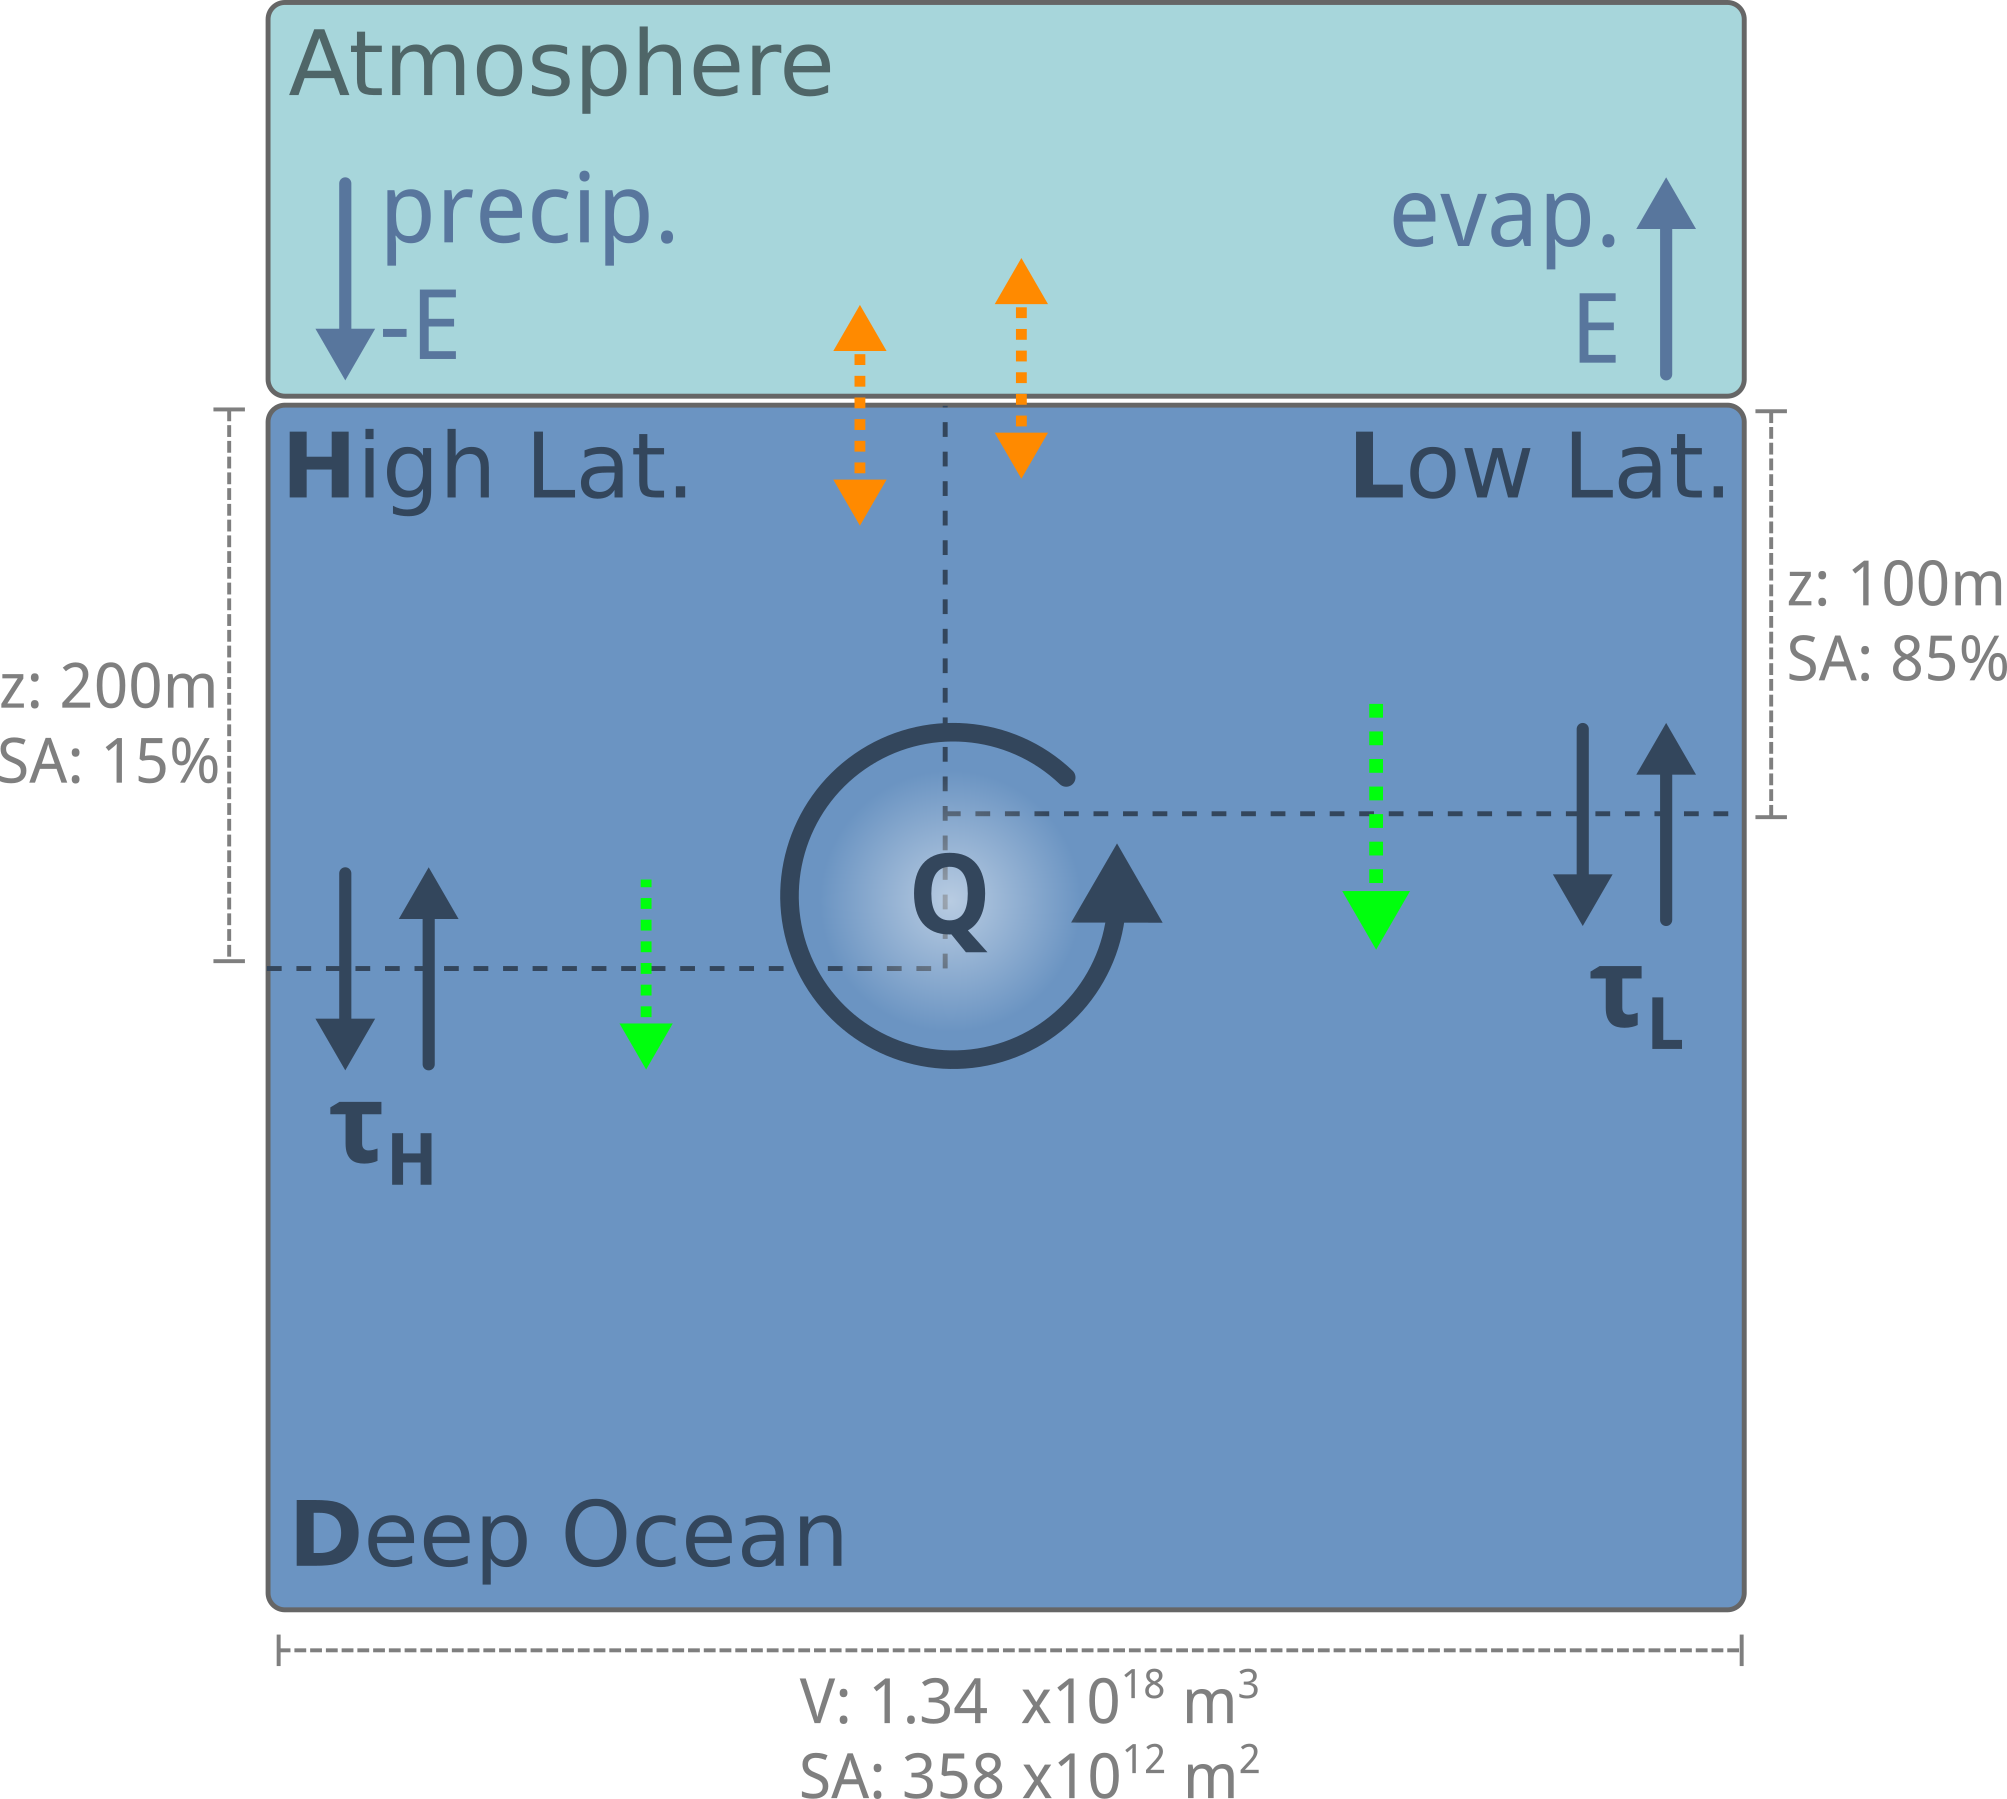
\includegraphics[width=\linewidth, totalheight=0.8\textheight, keepaspectratio]{ocean-3box-CO2-bio.png}
        
\end{frame}

\begin{frame}<handout:0>{Patterns of Ocean Carbon}
    \centering
    \slidereference{Sarmiento \& Gruber (2006)}

    \includegraphics<1>[width=\linewidth, totalheight=0.75\textheight, keepaspectratio]{carbon-ocean-atmos.png}

    \includegraphics<2>[width=\linewidth, totalheight=0.75\textheight, keepaspectratio]{carbon-cx-dic.png}
    \only<2>{
        \manualtext{\rotatebox{90}{$\mathrm{\upmu mol~kg^{-1}}$}}{0.52\linewidth}{-0.6}
    }

\end{frame}

\section{Organic Matter}

\begin{frame}{Phytoplankton}
    \centering

    \includegraphics<1>[width=\linewidth, totalheight=0.75\textheight, keepaspectratio]{seawifs-chlorophyll.png}
    \only<1>{\slidereference{SeaWIFS, NASA}}

    \only<2>{
    $$
    \mathrm{\underbrace{6 CO_2}_{carbon~dioxide} + \underbrace{6 H_2O}_{water} \xrightarrow[+light]{photosynthesis} \underbrace{C_6H_{12}O_6}_{glucose} + \underbrace{6 O_2}_{oxygen}}
    $$
    }

\end{frame}

\begin{frame}{Plankton}
    \centering

    \includegraphics<1>[width=\linewidth, totalheight=0.75\textheight, keepaspectratio]{carbon-plankton.jpg}
    \only<1>{\slidereference{Annegret Stuhr, GEOMAR}}

    \only<2>{\slidereference{@PlanktonPundit}}
    \includegraphics<2>[width=\linewidth, totalheight=0.75\textheight, keepaspectratio]{carbon-plankton-foodweb.jpeg}

\end{frame}

\begin{frame}{Organic Matter}

    \centering
    Organic matter is more than glucose - the organism requires nutrients to grow:

    \begin{align*}
    \mathrm{\underbrace{106 CO_2}_{carbon~dioxide} + \underbrace{16 NO_3 + H_3PO_4}_{nutrients} + 78 H_2O} &+ \mathrm{18H^+} & \\
    & \mathrm{ \xrightarrow[+light]{photosynthesis}} & \\
    && \mathrm{\underbrace{C_{106}H_{175}O_{42}N_{16}P}_{organic~matter} + \underbrace{150 O_2}_{oxygen}} \\
    \end{align*}

    \onslide<2|handout:1>{The main limiting nutrients are nitrate (\ce{NO3}) and phosphate \ce{PO4}.}

\end{frame}
 
\section{Nutrients}

\begin{frame}{Nutrient Requirements}
    \begin{columns}
        \begin{column}{0.4\linewidth}
            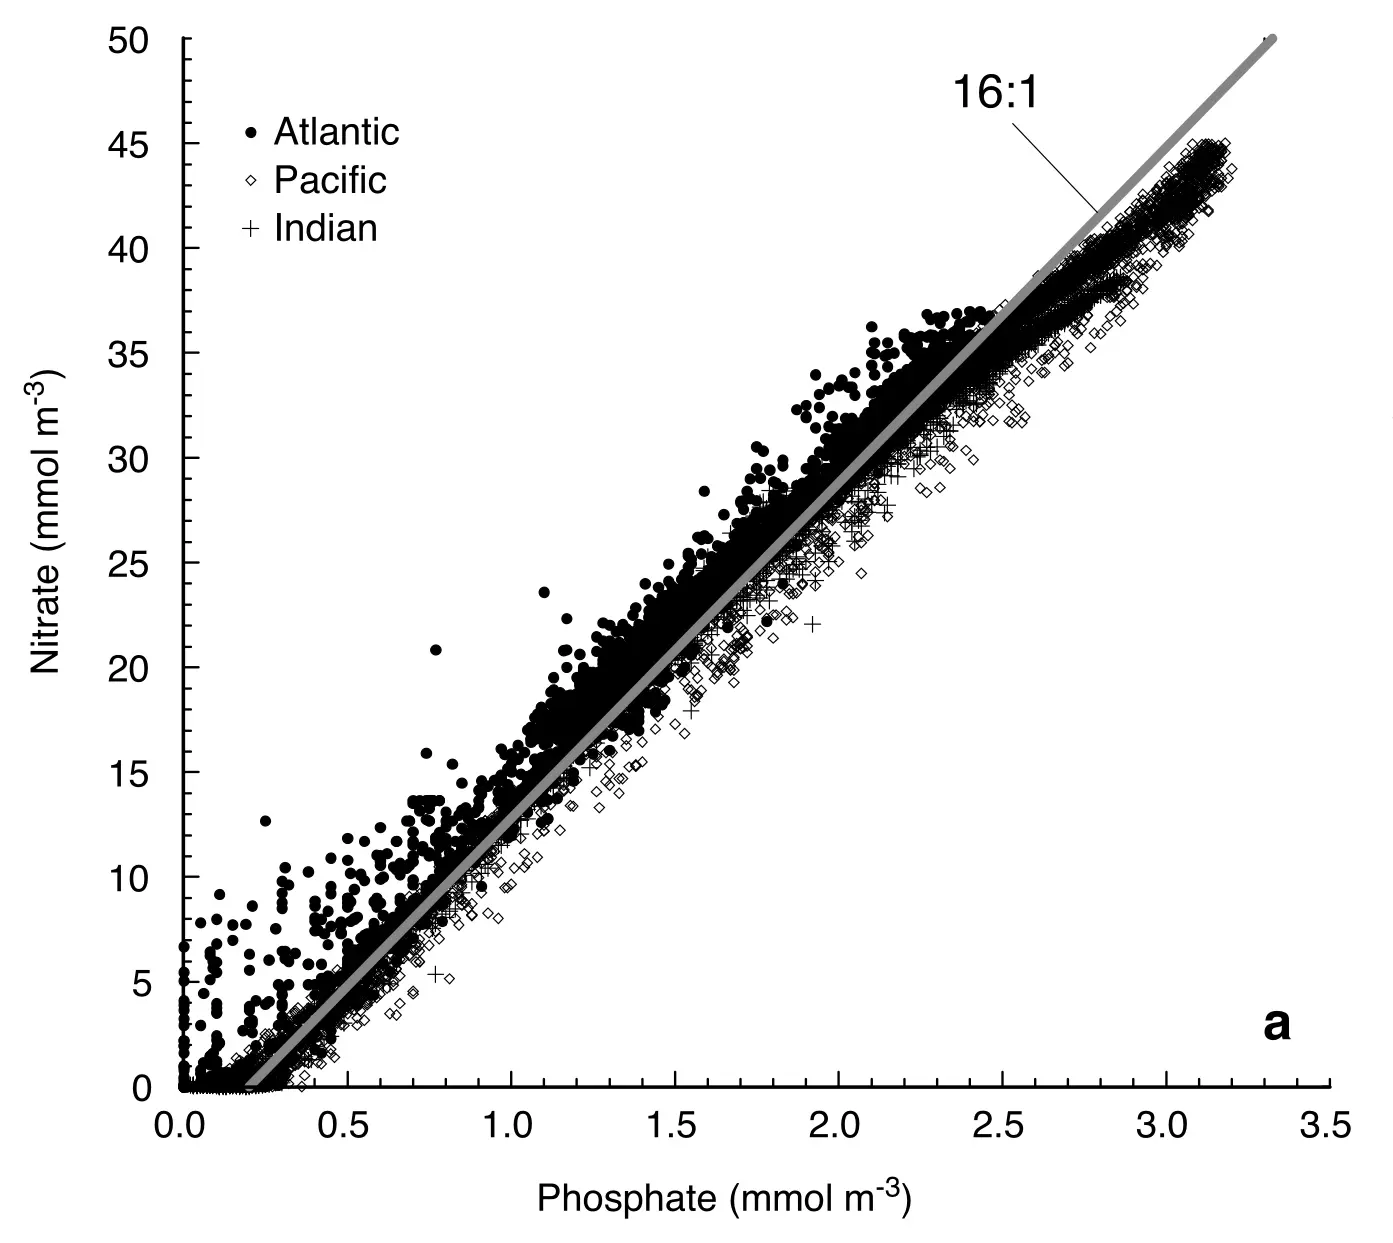
\includegraphics[width=\linewidth, totalheight=0.75\textheight, keepaspectratio]{carbon-redfield.png}
        \end{column}
        \begin{column}{0.5\linewidth}
            \begin{itemize}
                \item Organic matter contains a relatively constant ratio of C:N:P at 106:16:1.
                \item This is known as the \textbf{Redfield Ratio}.
                \item There is a tight coupling between the N:P ratio dissolved in the ocean and in organic matter.
            \end{itemize}
        \end{column}
    \end{columns}
\end{frame}

\begin{frame}{Nutrient Sources}
    \begin{itemize}
        \item \textbf{Phosphate} is derived from the dissolution of rocks on the continents. Supplied either via rivers, or by wind-blown dust from deserts.
        \item \textbf{Nitrate} also comes from terrestrial sources, but can also be captured from the air (\ce{N2}, 79\% of atmosphere) by specialised `nitrogen-fixing' phytoplankton.
    \end{itemize} 
\end{frame}

\begin{frame}{Nutrient Excess?}
    \centering
    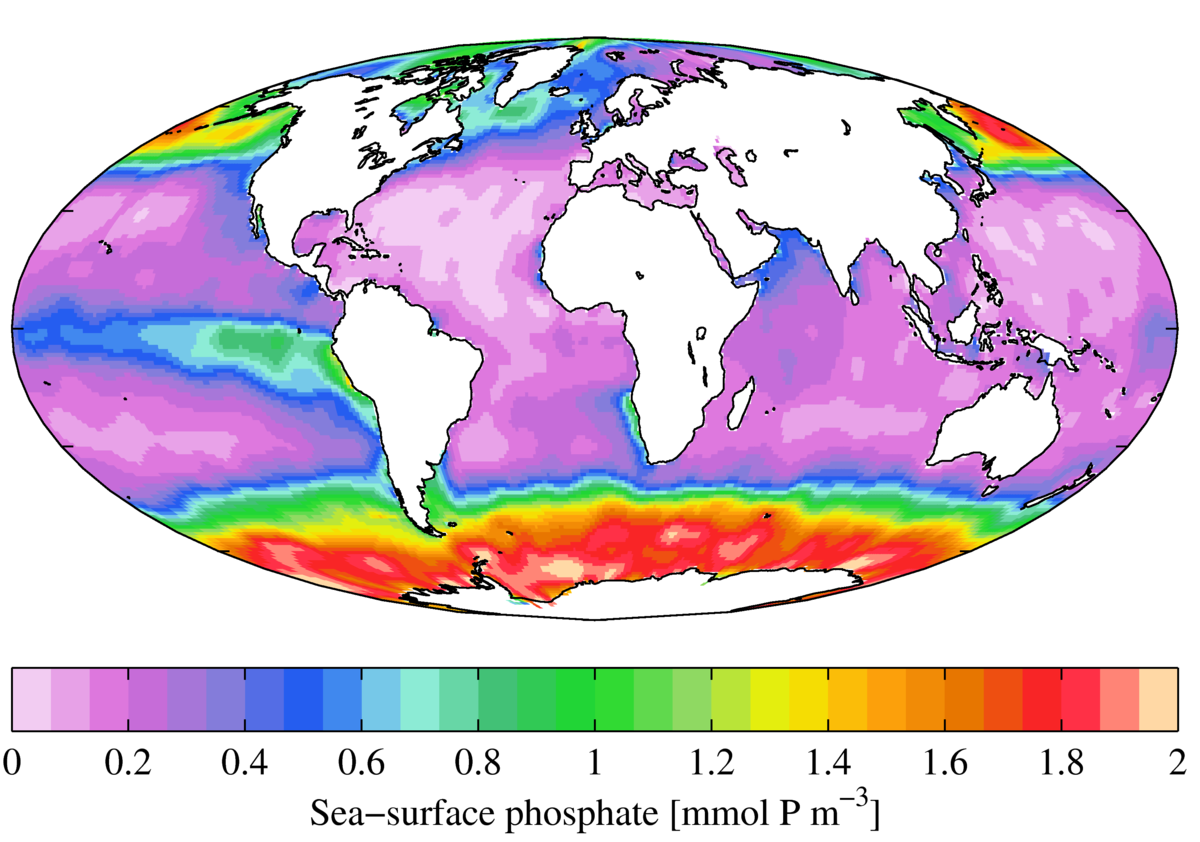
\includegraphics[width=\linewidth, totalheight=0.75\textheight, keepaspectratio]{ocean-surface-po4.png}
\end{frame}

\begin{frame}{Micronutrients}
    \centering
    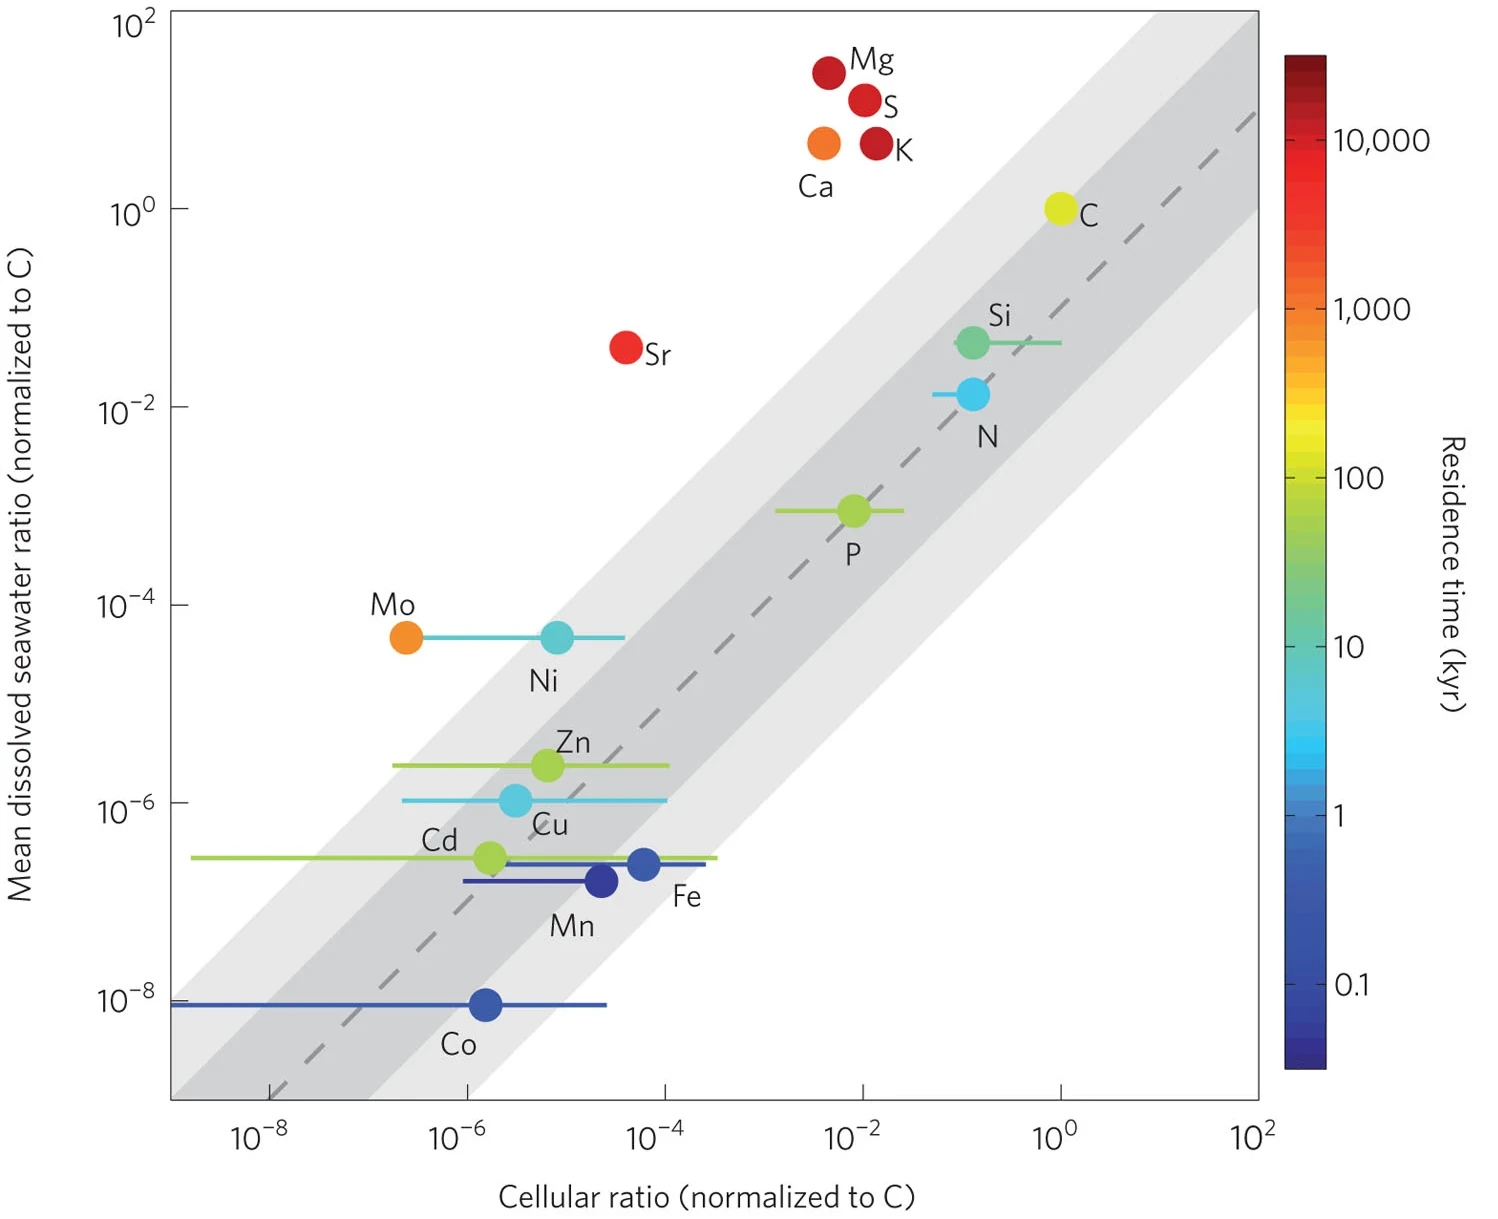
\includegraphics[width=\linewidth, totalheight=0.75\textheight, keepaspectratio]{carbon-nutrient-limitation.png}
\end{frame}

\begin{frame}{Nutrient Limitation}

    \begin{itemize}
        \item The availability of N, P limits phytoplankton growth.
        \item In some regions, micronutrients are also critical.
        \item For our model, we will use \ce{PO4} to limit phytoplankton growth.
    \end{itemize}

\end{frame}

\section{Light}

\begin{frame}{Light Limitation}
    \begin{columns}
        \begin{column}{0.7\linewidth}
            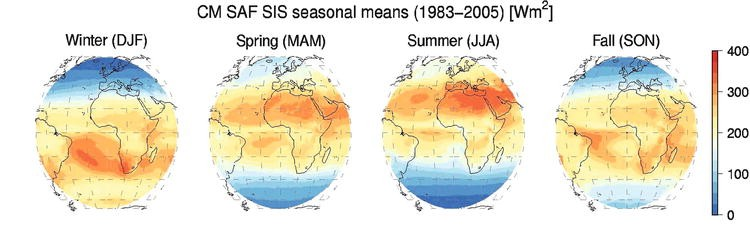
\includegraphics[width=\linewidth, totalheight=\textheight, keepaspectratio]{carbon-biopump-light.png}
        \end{column}
        \begin{column}{0.3\linewidth}
            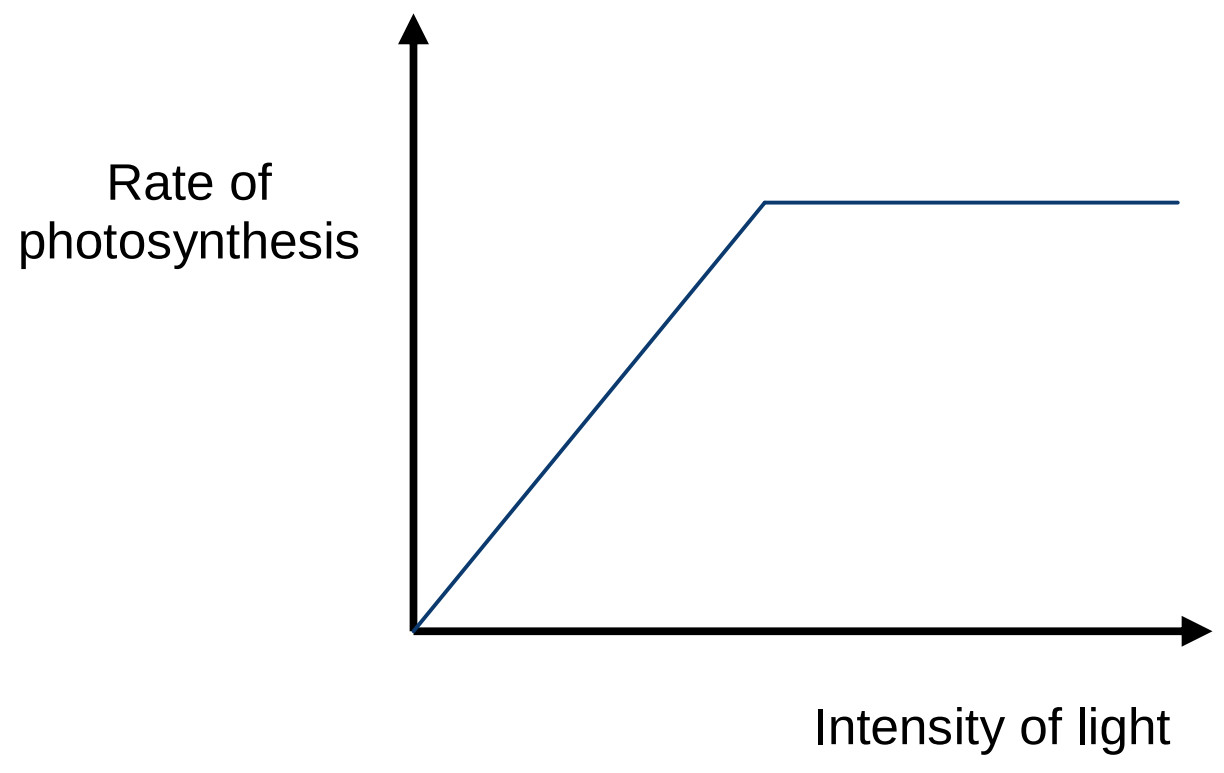
\includegraphics[width=\linewidth, totalheight=\textheight, keepaspectratio]{carbon-light-limitation.png}
        \end{column}
    \end{columns}
\end{frame}

\begin{frame}{Compensation Depth}
    \centering

    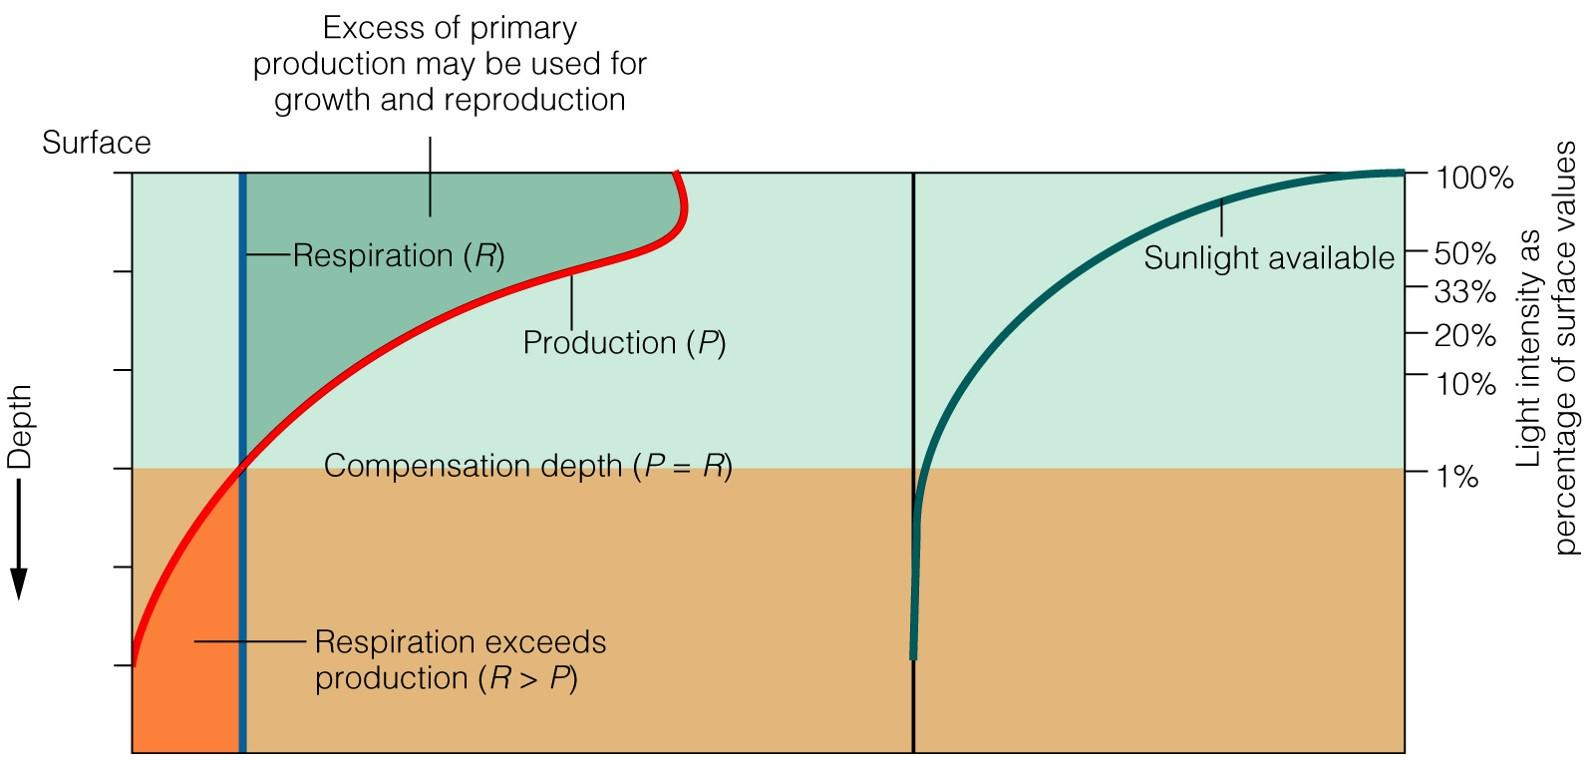
\includegraphics[width=\linewidth, totalheight=0.75\textheight, keepaspectratio]{carbon-compensation-depth.png}
\end{frame}

\begin{frame}{Approximating Light Limitation}
    \begin{itemize}
        \item The high latitudes are dark with a deep mixed layer depth (MLD) for part of the year.
        \item Nutrients accumulate in the winter months, and they spend longer in the surface waters.
        \item Nutrients have a longer lifetime ($\tau$) in the surface waters at high latitudes.
    \end{itemize}
\end{frame}

\section{Biological Pump}

\begin{frame}{Marine Snow}

    \only<1>{\slidereference{@PlanktonPundit}}
    \includegraphics<1>[width=\linewidth, totalheight=0.75\textheight, keepaspectratio]{carbon-plankton-foodweb.jpeg}

    \only<2|handout:0>{\slidereference{Sarmiento \& Gruber (2006)}}
    \includegraphics<2|handout:0>[width=\linewidth, totalheight=0.75\textheight, keepaspectratio]{carbon-npp.png}

    \only<3|handout:2>{
        \slidereference{Omand et al. (2020)}

        \begin{columns}
            \begin{column}{0.3\linewidth}
                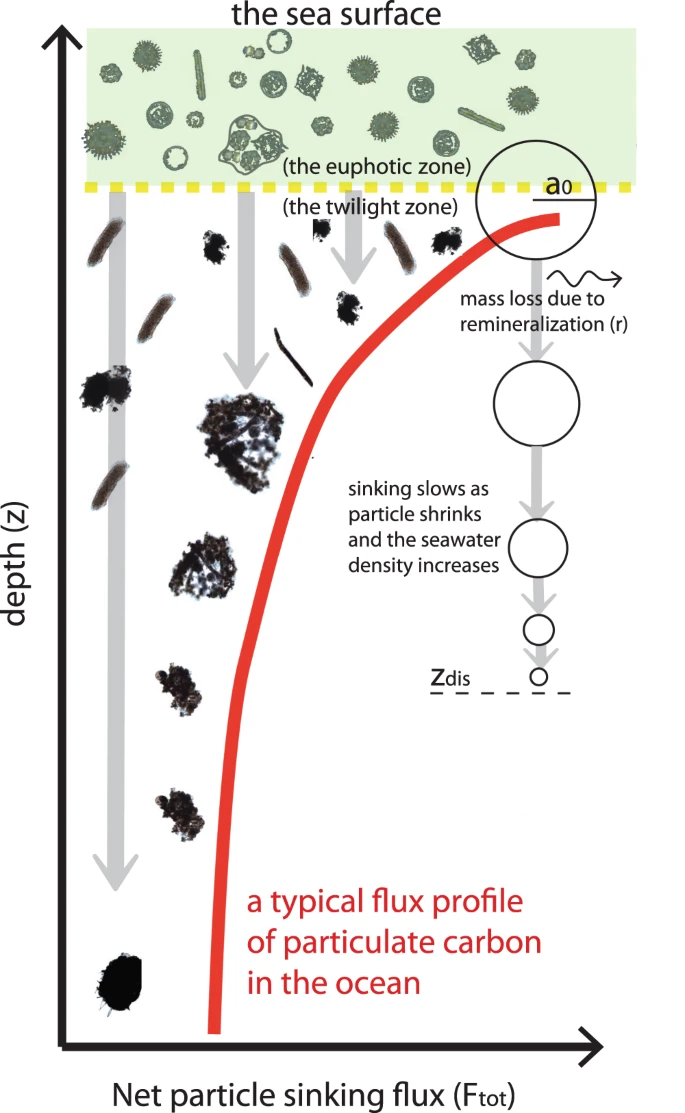
\includegraphics[width=\linewidth, totalheight=0.9\textheight, keepaspectratio]{carbon-particle-sinking.png}
            \end{column}
            \begin{column}{0.6\linewidth}
                \begin{itemize}
                    \item Organisms die and defecate, producing ``marine snow'' particles and aggregates.
                    \item Particles sink through the water column, and are `remineralised' by bacteria.
                    \item Remineralisation dissolves the particles back into the water column.
                    \item $\sim$80\% is remineralised in the surface ocean, $\sim$20\% is exported to the deep ocean.
                \end{itemize}
            \end{column}
        \end{columns}
    }

    \only<4|handout:3>{\slidereference{Sarmiento \& Gruber (2006)}}
    \includegraphics<4|handout:3>[width=\linewidth, totalheight=0.75\textheight, keepaspectratio]{carbon-poc-export.png}

\end{frame}

\begin{frame}{The Biological Pump}

    \centering

    \includegraphics<1|handout:0>[width=\linewidth, totalheight=0.65\textheight, keepaspectratio]{carbon-circ-6-biopump-const.png}

    \includegraphics<2|handout:0>[width=\linewidth, totalheight=0.65\textheight, keepaspectratio]{carbon-circ-7-biopump-deep.png}

    \includegraphics<3|handout:0>[width=\linewidth, totalheight=0.65\textheight, keepaspectratio]{carbon-circ-8-biopump-surf.png}

    \includegraphics<4|handout:1>[width=\linewidth, totalheight=0.65\textheight, keepaspectratio]{carbon-circ-9-biopump-full.png}

    \includegraphics<5|handout:2>[width=\linewidth, totalheight=0.75\textheight, keepaspectratio]{carbon-cx-po4.png}

    \includegraphics<6|handout:0>[width=\linewidth, totalheight=0.75\textheight, keepaspectratio]{carbon-cx-dic.png}

    \includegraphics<7|handout:3>[width=\linewidth, totalheight=0.75\textheight, keepaspectratio]{carbon-Csoft.png}


\end{frame}

\section{Modelling Ocean Carbon}

\begin{frame}{Modelling the Biological Pump}

    \begin{enumerate}
        \item Add a nutrient to limit biological productivity (\ce{PO4})
        \item Parameterise the link between photosynthesis, remineralisation and carbon chemistry.
    \end{enumerate}

\end{frame}

\begin{frame}{1. Adding a Nutrient}

    \ce{PO4} is onsumed by phytoplankton and remineralised at depth. 
    
    Describe uptake and export with $\tau^P$, which will be longer in high latitudes because of light limitation. Note that $\tau^P$ is \textit{not} production, but \textit{export} - how much of the organic matter produced by phytoplankton leaves the surface and enters the deep ocean.

    \begin{align*}
        \mathrm{\dv{P_L}{t}} &= \mathrm{[\mathrm{transport}] - \frac{1}{\tau^P_L} P_L} \\
        \mathrm{\dv{P_H}{t}} &= \mathrm{[\mathrm{transport}] - \frac{1}{\tau^P_H} P_H} \\
        \mathrm{\dv{P_D}{t}} &= \mathrm{[\mathrm{transport}] + \left. \left( \frac{V_L}{\tau^P_L} P_L + \frac{V_L}{\tau^P_H} P_H \right) \middle/ V_D \right.}
    \end{align*}

\end{frame}

\begin{frame}{2. Coupling productivity and Carbon}

    Photosynthesis and remineralisation affect both DIC and TA, and can be simplified to:

    $$
    \mathrm{P + 106 DIC - 18 TA \xrightleftharpoons[remineralisation]{photosynthesis} [organic~matter]}
    $$

    We can link DIC and TA to PO4 via the Redfield Ratio as:

    \begin{align*}
        \mathrm{\frac{d[DIC]_{bio}}{dt}} &= \mathrm{106 \frac{dP_{bio}}{dt}} \\
        \mathrm{\frac{d[TA]_{bio}}{dt}} &= \mathrm{-18 \frac{dP_{bio}}{dt}}
    \end{align*}

    Which we include alongside transport and atmospheric echange\dots

\end{frame}

\begin{frame}{2. Coupling productivity and Carbon}

\begin{align*}
    \mathrm{\dv{DIC_L}{t}} &= \mathrm{\begin{bmatrix} \mathrm{transport} \\ \mathrm{CO_2~exch.}\end{bmatrix} - 106 \frac{1}{\tau^P_L} P_L} \\
    \mathrm{\dv{DIC_H}{t}} &= \mathrm{\begin{bmatrix} \mathrm{transport} \\ \mathrm{CO_2~exch.}\end{bmatrix} - 106 \frac{1}{\tau^P_H} P_H} \\
    \mathrm{\dv{DIC_D}{t}} &= \mathrm{[\mathrm{transport}] + \left. \left( 106 \frac{V_L}{\tau^P_L} P_L + 106 \frac{V_H}{\tau^P_H} P_H \right) \middle / V_D \right.}
\end{align*}

\begin{align*}
    \mathrm{\dv{TA_L}{t}} &= \mathrm{[\mathrm{transport}] + 18 \frac{1}{\tau^P_L} P_L} \\
    \mathrm{\dv{TA_H}{t}} &= \mathrm{[\mathrm{transport}] + 18 \frac{1}{\tau^P_H} P_H} \\
    \mathrm{\dv{TA_D}{t}} &= \mathrm{[\mathrm{transport}] - \left. \left( 18 \frac{V_L}{\tau^P_L} P_L + 18 \frac{V_H}{\tau^P_H} P_H \right) \middle / V_D \right.}
\end{align*}

\end{frame}

\end{document}


% \begin{frame}{TITLE}
% \end{frame}